\chapter{Introduction}

% the code below specifies where the figures are stored
\ifpdf
    \graphicspath{{1_introduction/figures/PNG/}{1_introduction/figures/PDF/}{1_introduction/figures/}}
\else
    \graphicspath{{1_introduction/figures/EPS/}{1_introduction/figures/}}
\fi

\section{Overview}
Computers have been widely used in music performances for many years. Some
advanced systems use the computer as a independent module to replace a
single instrument in an orchestra. In popular music computers have proved
to be particularly successful. Both classical and popular music have many
opportunities for innovative applications used by highly intelligent and
coordinated computer music systems. With more powerful algorithms and more
advanced sensing devices, computer music systems have the potential to
replace musicians. In the future, computer music systems will inspire new 
musical directions based on new
capabilities and generate new concepts from new technologies.

Live popular music offers a wealth of opportunities for computing and music
research.  We refer to the integration of computers as independent autonomous
performers into popular live music performances as Human Computer Music
Performance (HCMP). In HCMP, computers become more than instruments and are,
to some degree, seen as performers. To bring HCMP into the realm of popular
music performance, certain problems need to be solved. 

One problem is that
popular music is organized around a tight synchronization to beats, and a
computer cannot reliably and efficiently adapt to human tempo variations.
Another significant problem is that an HCMP project is a large complex
system which contains many components, each one relying on the cooperation of several
different subcomponents to complete its task.

The motivation behind the HCMP Player is to provide a good solution to these
problems. When successful, the HCMP Player will display different
representations of music, work as an accompanist and quickly adjust its
tempo to follow the performer. A clearly defined programming interface is
also required in order to foster communication and cooperation with all
components within the system. To create such a player, we must coordinate
time between different media. We need at least two functional components,
one component working as ``backend'' and responsible for coordinating and
scheduling different music events, the other, working as ``frontend'', will
receive commands from the user or other components and dynamically adjust
play sequences and tempo based on those requests.

This paper begins with the role of the HCMP Player in the HCMP project. Then
the ``big picture of'' of the HCMP project will be discussed, followed by a
presentation of the individual HCMP components. Finally the question of how
the HMCP Player fits into the whole picture will be addressed. In the
following three chapters design issues with the HCMP Player are addressed.
Each chapter approaches the problem from a different perspective. Chapter 2
describes the design of Graphical User Interface (GUI) for the HCMP Player together
with a detailed explanation of all the GUI components' usage and function.
Chapter 3 describes the ``backend'' of the HCMP Player - the player engine,
and illustrates how the player engine cooperates and communicates with the
GUI to complete external requests. Chapter 4 addresses the network
communication problem between multiple players. A API is
defined to integrate the HCMP Player with other components in the HCMP
project.  Chapter 5 describes the implementation details of the HCMP Player
and includes pseudocode to provide a clear explanation of this. Chapter 6
focuses on the evaluation of the HCMP Player. A full list of features
will be given and a clear success criteria used to evaluate the HCMP Player
will be defined. In Chapter 7, I summarize my work and propose possible
future works.

\section{Background}

Before making a formal introduction to the background of HCMP Player, 
I would like to make a short review of  
some existing human computer music systems. The most common use of computers in
music performance is in computer instruments, typically keyboards.
These, and other electronic instruments, are essentially substitutes for traditional
instruments and rely upon human musicians for their control and coordination with
other musicians. 

Many composers of interactive contemporary art music use computers
to generate music in real time, often in response to live performers.
These systems are rarely capable of synchronizing to rhythmic playing
so these techniques are not very useful for traditional or popular music 
forms.

Another use of the computer in music is in computer accompaniment systems 
\cite{Roger:89}, 
whcih solve the synchronization problem by assuming a pre-determined 
score (music notation). During the performance, a performer expressively 
plays music score while the accompaniment system ``listens'' and make a analysis, 
then follows the performer 
in the score and synchronizes an accompaniment.

In live popular music peformance, computers can be quite useful too.
The computer has had a significant
impact on popular music through drum machines, sequencers and loop-based
interfaces, but one can argue that popular music has adapted to new technology
rather than the other way around. The sound and beat of drum machines seems stiff,
mechanical, and monotonous to many musicians, but that became the trance-like
foundation of club dance music and other forms. Similarly, 
the inability of
sequencers and other beat-based software to “listen” to human musicians has led to
performances with click tracks in fixed media or simply a fixed drum track that live
musicians must follow. Ableton Live \cite{Ableton:2011} is an example of software that
uses a beat, measure, and section framework to synchronize music in live
performance, but the program is not well suited to adapting to the tempo of live
musicians. Robertson and Plumbley \cite{Robertson:2007} used a real-time beat 
tracker in
conjunction with Ableton Live software to synchronize pre-recorded music 
to a live drummer. This extension could be considered HCMP.
Table 1.1 summarizes some existing computer music systems and their usage.

\begin{table}[htdp]
\centering
\begin{tabular}{| p{5cm} | p{8cm} |} % ccc means 3 columns, all centered; alternatives are l, r

\hline
Computer Instruments & Direct physical interaction with virtual instruments \\

\hline 
Interactive Contemporary Art Music & Composed interactions; often unconstrained by
traditional harmony or rhythm.\\

\hline
Computer Accompaniment & score following synchronizes computer to live performer.\\

\hline
Fixed Media  & Many musical styles and formats. Live performers
synchronize to fixed recording.\\

\hline
Conducting System & Synchronize live computer performance by tapping or
gesturing beats. Best with “expressive”
traditional/classical music.\\
\hline
\end{tabular}
\caption[Computer Music Systems Summary]{Computer Music Systems Summary}
\label{latexin_genes} % label for cross-links with \ref{latexin_genes}
\end{table}

\section{Objective}
The objective of HCMP \cite{Dawen:2011} is to create an autonomous 
``artificial performer'' with the ability of a human musical performer. 
Ideally, HCMP should not require a human operator instead, the system itself 
be adaptive and responsive. With a sophisticated listening and sensing
component, HCMP is able to adjust system parameters in real-time during 
performance. 

From a functional perspective, we can divide HCMP into two main
categories: music preparation and music performance. The music preparation
part aims to work with and understand multiple music representations in order
to prepare material for performance. The music
performance part deals with music.     

An important component of the music performance part is the HCMP Player, 
which is able to flexibly  
adjust and respond to changes of music signal. Figure 1 illustrates the relationship 
between the scheduler, conductor and HCMP Plyaer. During performance, the HCMP Player will 
be controlled by conductor and constantly receive control messages 
from the conductor. In this project, I have designed, and implemented the HCMP midi player 
for the HCMP project.
\begin{figure}[H] % Example image
\center{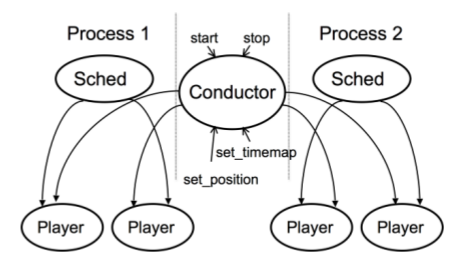
\includegraphics[width=0.65\linewidth]{1/1.png}}
\caption{Key Components of HCMP}
\label{fig:speciation}
\end{figure}
 

\section{HCMP Player Architecture}
The HCMP Player is mainly made up of two threads, that we call the GUI thread 
and the performer thread. The GUI thread takes care of user input, maintaining 
graphic state. The performer thread plays MIDI file synchronously with other 
players, each thread is an independent 
module. The two threads communicate with each other through a pair of shared 
message queues. We assume the message 
queue is large enough to avoid blocking by thread. The performer thread
handles time-critical operations, and there will be a timer setup 
before this thread is created. The goal of the timer is to 
wake up the performer thread periodically. Everytime the performer 
thread's timer callback function is invoked, 
it will check the message queue and process any command from the control thread.
Figure 2 illustrates the overall structure of the Player.

\begin{figure}[H]
\center{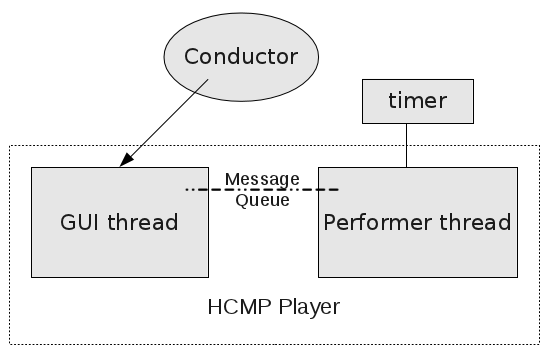
\includegraphics[width=0.65\linewidth]{2/2.png}}
\caption{Architecture of the HCMP Midi Player}
\label{fig:speciation}
\end{figure}

During the performance, the HCMP Player will act as 
the server for the conductor component, which is constantly 
receiving control messages and responding accordingly. The
conductor receives and forwards message to start and stop playing,
set the position, and change the tempo.

%Most organisms use polymers of glucose units for energy storage and differ only slightly in the way they link together monomers to sometimes gigantic macromolecules. Dextran of bacteria is made from long chains of $\alpha$-1,6-linked glucose units. 

%: ----------------------- HELP: special characters
% above you can see how special characters are coded; e.g. $\alpha$
% below are the most frequently used codes:
%$\alpha$  $\beta$  $\gamma$  $\delta$

%$^{chars to be superscripted}$  OR $^x$ (for a single character)
%$_{chars to be suberscripted}$  OR $_x$

%>  $>$  greater,  <  $<$  less
%≥  $\ge$  greater than or equal, ≤  $\ge$  lesser than or equal
%~  $\sim$  similar to

%$^{\circ}$C   ° as in degree C
%±  \pm     plus/minus sign

%$\AA$     produces  Å (Angstrom)

% dextran, starch, glycogen continued
%Starch of plants and glycogen of animals consists of $\alpha$-1,4-glycosidic glucose polymers \cite{lastname07}. See figure \ref{largepotato} for a comparison of glucose polymer structure and chemistry. 

%Two references can be placed separated by a comma \cite{lastname07,name06}.

%: ----------------------- HELP: references
% References can be links to figures, tables, sections, or references.
% For figures, tables, and text you define the target of the link with \label{XYZ}. Then you call cross-link with the command \ref{XYZ}, as above
% Citations are bound in a very similar way with \cite{XYZ}. You store your references in a BibTex file with a programme like BibDesk.



%\figuremacro{largepotato}{A common glucose polymers}{The figure shows starch granules in potato cells, taken from \href{http://molecularexpressions.com/micro/gallery/burgersnfries/burgersnfries4.html}{Molecular Expressions}.}

%: ----------------------- HELP: adding figures with macros
% This template provides a very convenient way to add figures with minimal code.
% \figuremacro{1}{2}{3}{4} calls up a series of commands formating your image.
% 1 = name of the file without extension; PNG, JPEG is ok; GIF doesn't work
% 2 = title of the figure AND the name of the label for cross-linking
% 3 = caption text for the figure

%: ----------------------- HELP: www links
% You can also see above how, www links are placed
% \href{http://www.something.net}{link text}

%\figuremacroW{largepotato}{Title}{Caption}{0.8}

% variation of the above macro with a width setting
% \figuremacroW{1}{2}{3}{4}
% 1-3 as above
% 4 = size relative to text width which is 1; use this to reduce figures


%Insulin stimulates the following processes:
%
%\begin{itemize}
%\item muscle and fat cells remove glucose from the blood,
%\item cells breakdown glucose via glycolysis and the citrate cycle, storing its energy in the form of ATP,
%\item liver and muscle store glucose as glycogen as a short-term energy reserve,
%\item adipose tissue stores glucose as fat for long-term energy reserve, and
%\item cells use glucose for protein synthesis.
%\end{itemize}

%: ----------------------- HELP: lists
% This is how you generate lists in LaTeX.
% If you replace {itemize} by {enumerate} you get a numbered list.

%: ----------------------- HELP: tables
% Directly coding tables in latex is tiresome. See below.
% I would recommend using a converter macro that allows you to make the table in Excel and convert them into latex code which you can then paste into your doc.
% This is the link: http://www.softpedia.com/get/Office-tools/Other-Office-Tools/Excel2Latex.shtml
% It's a Excel template file containing a macro for the conversion.

% There you go. You already know the most important things.
